\documentclass[a4paper,10pt]{scrartcl}
\usepackage[utf8]{inputenc}
\usepackage{graphicx}
\usepackage{float}

% Title Page
\title{Codmon: A multi-platform modular test environment.}
\author{Berend van Veenendaal}
\bibliographystyle{plain}
%hieronder wordt de project naam als variabele gedeclareerd
\newcommand{\project}{Codmon 2.0}
\newcommand{\CS}{C\nolinebreak\hspace{-.05em}\raisebox{.6ex}{\bf \#}}

\begin{document}
\maketitle

\begin{abstract}
TODO:Abstract
\end{abstract}
\newpage
\section*{Preface}
\label{sec:Preface}
TODO: Preface,acknowledgements
\newpage
\tableofcontents
\newpage

\section{Introduction}
\label{sec:Introduction}
This chapter will give an introduction about the \project{} project by giving a brief decription of background of my research and of the
previous version of the Codmon project. It also describes the structure of this thesis.

\subsection{Background}
\label{sec:Background}
In times when software projects become more and more complex, testing of this software becomes more and more important. Many software
related problems are caused by lack of testing of the software~\cite{TTCST}. One of the challenges of software engineering is to make
sure that the software behaves in the same way on different platforms. Even when software is written in such a way that it can run on multiple platforms, there 
are still issues that must be dealt with, before one is able to run and test the software. Example issues are the configuration of the test environment 
or finding and installing all the prerequisite libraries etc etc. 

\subsection{Problem indication}
\label{subsec:Problemindication}
Nowdays there are numerous test frameworks and test environments available. For example there is \emph{Junit}\cite{Junit} for Java-unit testing and \emph{NUnit}\cite{Nunit} for \CS{}-unit testing.
There are also different environments like Hudson\cite{HudsonDoc}, \cite{Hudson}, Jenkins\cite{JenkinsDoc} which can build a project and run a series of (unit) tests against this project. 
All of the frameworks and environments have both their advantages and disadvantages. One of the advantages of unit testing is that a software developer easily can add new \emph{functional} unit tests.
One of the disadvantages is that standard unit testing ignores non-functional tests like performance testing and the deployment of the software. Jenkins and Hudson,like Unit tests, also have their
disadvantages. One of them is, although they both run on different platforms, in their usage they are not really platform independent. For example, if you want
to make a connection from Hudson or Jenkins to a remote machine you do this by executing a shell script to be able to do this, a user must know in advance on which platform this script has to run.
With this in mind you can see that, although it is possible to connect to different machines it is not a 100\% platform independent environment.
 
\subsection{Problem statement}
\label{subsec:Problemstatement}
The test frameworks and test environments mentioned in section \ref{subsec:Problemindication} can be criticized on one or more aspects. What we are looking for is in fact, a combination
of the positive aspects of the described frameworks and environments, without the undesirable aspects. So the central question is, is it possible to design a
multi-platform, modular test environment? In addition, we study if it is possible to design the test environment in a \emph{user friendly} way, meaning that it must
be possible to easily add both new test cases and software without knowing anything about the internal mechanisms of the test environment.\\

\noindent This thesis describes a multi-platform, user friendly modular test environment called \project{}. The \project{} project provides users with a set of virtual machines,
in which \project{} is already installed and preconfigured. The purpose of the virtual machines is to make it as user friendly as possible. By doing it this way the only tasks
a \project{} user has to do are 1) add their project  to the init.xml file. and 2) add the tests to a so called wrapper file. Both of these files will be discussed in more detail in 
sections \ref{subsec:init} and \ref{subsec:wrappers} .


\subsection{Thesis outline}
\label{subsec:Thesisoutline}
Section \ref{sec:codmon} first describes the current Codmon framework. It starts with explaining why the original Codmon was built. Then it continuous with a description of the design of Codmon
and the problems of the current Codmon project in section \ref{sec:codmon}. Section \ref{sec:Codmon2.0} describes the \project{} project. This section starts with the \emph{The road 
to \project{}}. Here we explain the ideas that came into mind and how we got to the final \project{} design. Section \ref{sec:Codmon2.0} describes the \project{} project. It starts with 
a general description of the project followed by a detailed explanation of the different modules of \project{}. In Section \ref{sec:conclusion} we discuss the results based on section \ref{sec:experiments}. We end this section with a brief discussion of related work.

\newpage

\section{Codmon}
\label{sec:codmon}
Before we start describing the \project{} we start with a description of the current Codmon framework, we first describe How Codmon works and why it is not good enough for the purposes mentioned
in section \ref{subsec:Problemstatement}. The original Codmon framework was built in 2005 by François Lesuer\cite{Codmon}. Codmon is built for testing Ibis projects\cite{Ibis}\cite{Satin}\cite{MPJ}\cite{IPL}\cite{GMI} 
on the DAS-2\cite{das2} computer. Codmon was (At this moment the das2 and Codmon aren't in use anymore) able to perform both functional and performance tests. If for some reason a particular
test failed, Codmon reported the problems directly to the programmer who made the last changes in code under test. It was also the intention that Codmon would be extensible. In this the Codmon 
developers succeeded only partially. We will discuss this more in depth in section \ref{subsec:CodmonProblems}.  

\subsection{Codmon Design}
\label{subsec:CodmonDesign}
This section we will describe the design of the Codmon framework. The setup of Codmon is more or less modular and consiste of a few core parts. The set of tests that should run is describe
in different configuration files which are called \emph{Sensors}. A sensor describes which test should be executed and also the software that is under these tests. A sensor consits of two
parts. First there is the \emph{onoff} part, which is used for compilation parts and functional tests. The core of each sensor element in a sensor file consists of two parts: a wrapper and
a shell-script command. Second there is the \emph{graph} part. This part is used for performance tests. The results of a performance test will be compared with the results of previous tests 
and if the performance result of a test drops below a certain level, an alarm is raised. The same occures when one or more functional tests are failing.\\

\noindent Where a \emph{sensor} describes the structure of a set of tests, a so called \emph{wrapper} describes an actual test. Wrappers are small programms that are written int the PERL
language. The return value of a wrapper indicates if a test succeeded or not. In case of a failure an alarm is raised and both the return value and the actual error code will be shown to
the programmer who made the last contribution to the code. The results of the performance tests are plotted in a graph, which makes it easy for the developers to see the performance
behaviour. Figure 1 shows a schematic picture of the Codmon structure. More technical details about the Codmon implementation can be found in \cite{Codmon}

\begin{figure}[!ht]
  \caption{\emph{figure 1: Codmon}}
  \centering
    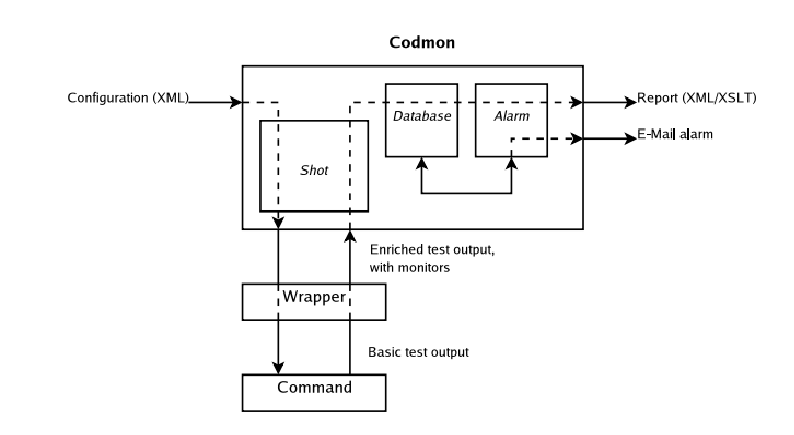
\includegraphics[scale=0.5]{codmon}
\end{figure}



\subsection{Codmon problems}
\label{subsec:CodmonProblems}
The purpose of this research was to see if it's possible to design a multi-platform, user friendly modular test environment. There are multiple reasons why Codmon doesn't satisfy this. First
to be multi-platform, without applying every change multiple times, the platform must be written in a platform-independent language. If we take a look ad Codmon there are at least three 
different lang used. The core of Codmon is written in java, which is indeed platform independent\cite{Java}, so this is not the real problem. As we've explained in section \ref{sec:codmon} the
important part of the sensors is a combination of a \emph{shel-script} command and a \emph{wrapper}

TODO: Was only supporting cvs. difficult to extend for other users.
TODO: Think about too many different languages and techniques (java , perl) the later isn't platform independent.


\newpage
\section{\project{}}
\label{sec:Codmon2.0}

\subsection{the road to \project{}}
//TODO: Think of better subsection title!!
//TODO: Explain ideas and road to solution

\subsubsection{The init.xml file}
\label{subsec:init}

\subsubsection{Version control}
\label{subsec:versionControl}

\subsubsection{wrappers}
\label{subsec:wrappers}

\subsection{experiments}
\label{sec:experiments}

\newpage

\section{Conclusion and related work}
\label{sec:conclusion}
TODO: give answers to the questions from section Problem statement
TODO: Discus related future work
\newpage

\bibliography{Master}
\end{document}    